\section{Realisation}
\subsection{Engineering work}
My work was split into many different parts. I made a \brand{GitHub} deposit : \url{https://github.com/jcelerier/spectral-subtraction} in which there are folders that correspond to these parts.
\subsubsection{Implementation of the algorithms}
This part will refer to the folder \texttt{libnoisered}. 

\paragraph{Technologies used}
As soon as I could, I tried to make the algorithms as a separate library, which has for sole dependencies \ac{FFTW} and \brand{CWTLIB++}. A corresponding \brand{Doxygen} documentation can be generated inside this folder, or by calling \texttt{make doc} on the root of the repository.

\subparagraph{Choice of \ac{FFTW}} I choose to use \ac{FFTW} because it seems that it is one of the best performing Fourier Transform, apart from implementations which are devised specially towards a particular \brand{CPU}: \url{http://www.fftw.org/speed/}.
It also supports the \brand{NEON} vectorial instructions of the \brand{ARM} processor, which can provide a performance boost.
\subparagraph{Overlap-add technique}
One of the technique used here is the overlap-add technique. Instead of performing a Fourier transform on a data-filled array, the input array is twice the data size, and its second half is filled by zeros.
After the subtraction is applied, the output array's first half is added to the previous array's last half, and so on. This is the only point on the algorithms that can't be threaded easily.
Overlap-add method can be enabled or disabled. If it is disabled, a simple rectangular window is used.
\paragraph{Spectral Subtraction}
The numerical algorithms are most of the time very straightforward.

\begin{algorithm}
 \SetAlgoLined
 \KwData{A signal spectrum X, a noise estimation Z}
 \KwResult{A new signal X' with less noise}

 \ForAll{bands $i$ in the spectrum}{
	$ t_0\gets \power(X_i)$ \\
	$ t_1 \gets t0 - \alpha * Z(i)$ \\
	$ t_2 \gets \beta * t0$ \\
	$ \mathrm{mag} \gets \sqrt{\max(t1, t2)}$ \\
	$ \mathrm{ph} \gets \phase(X_i)$ \\
	$ X_i \gets \recompute(mag, ph)$ 
	\tcp{Spectrum is given in complex format}
 }
 \caption{Simple spectral subtraction (\texttt{subtraction/simple\_ss.cpp})}
\end{algorithm}

Whenever I could, I tried to use \brand{C++ STL} algorithms, like \texttt{std::transform}, or \texttt{std::accumulate}.
There are several advantages : 
\begin{itemize}
\item They make the code very concise and readable. For instance, here is the code that computes the power for every band of a spectrum array, in complex format : 
\begin{lstlisting}[caption=math\_util.cpp]
void compute_power(fftw_complex *in, double *powoutput, unsigned int size)
{
	std::transform(in, in + size, powoutput, ToPower);
}
\end{lstlisting}

Here, \texttt{ToPower} is a \brand{C++11} lambda expression, which is used in other functions as well :
\begin{lstlisting}[caption=math\_util.cpp]
auto ToPower = [&] (fftw_complex val)
{
	return std::pow(val[0], 2) + std::pow(val[1], 2);
};
\end{lstlisting}
I choose to use a lambda-expression because common compilers seems to optimize them better than ordinary functions\cite[p.~213]{cppstl}, and here performance is critical.
\item The \brand{C++} standard imposes a maximal complexity for these algorithms. For instance, \texttt{std::max} must be in $\theta(n)$ (courtesy of \url{www.cplusplus.com}).
\item They present the advantage of having parallel versions, when using \brand{GCC}. These versions are enabled with a single \brand{G++} flag : \texttt{D\_GLIBCXX\_PARALLEL}. This way, they can be easily disabled for the embedded board, where it is inefficient because it is single-threaded, while they can be enabled when doing tests on the computer. 
\end{itemize}


\paragraph{First organisation}
At first, when there were only a few algorithms to code, it seemed logical to have a class only for noise estimation algorithms, and a class only for subtraction algorithms. However, some algorithms like the one proposed by Rainer Martin\cite{martin2001noise} uses a lot of static variables and tables, because data has to be kept from a frame to another. 
Here was the first class diagram : 
\begin{figure}[H]
\begin{center}
\hspace{-11em}
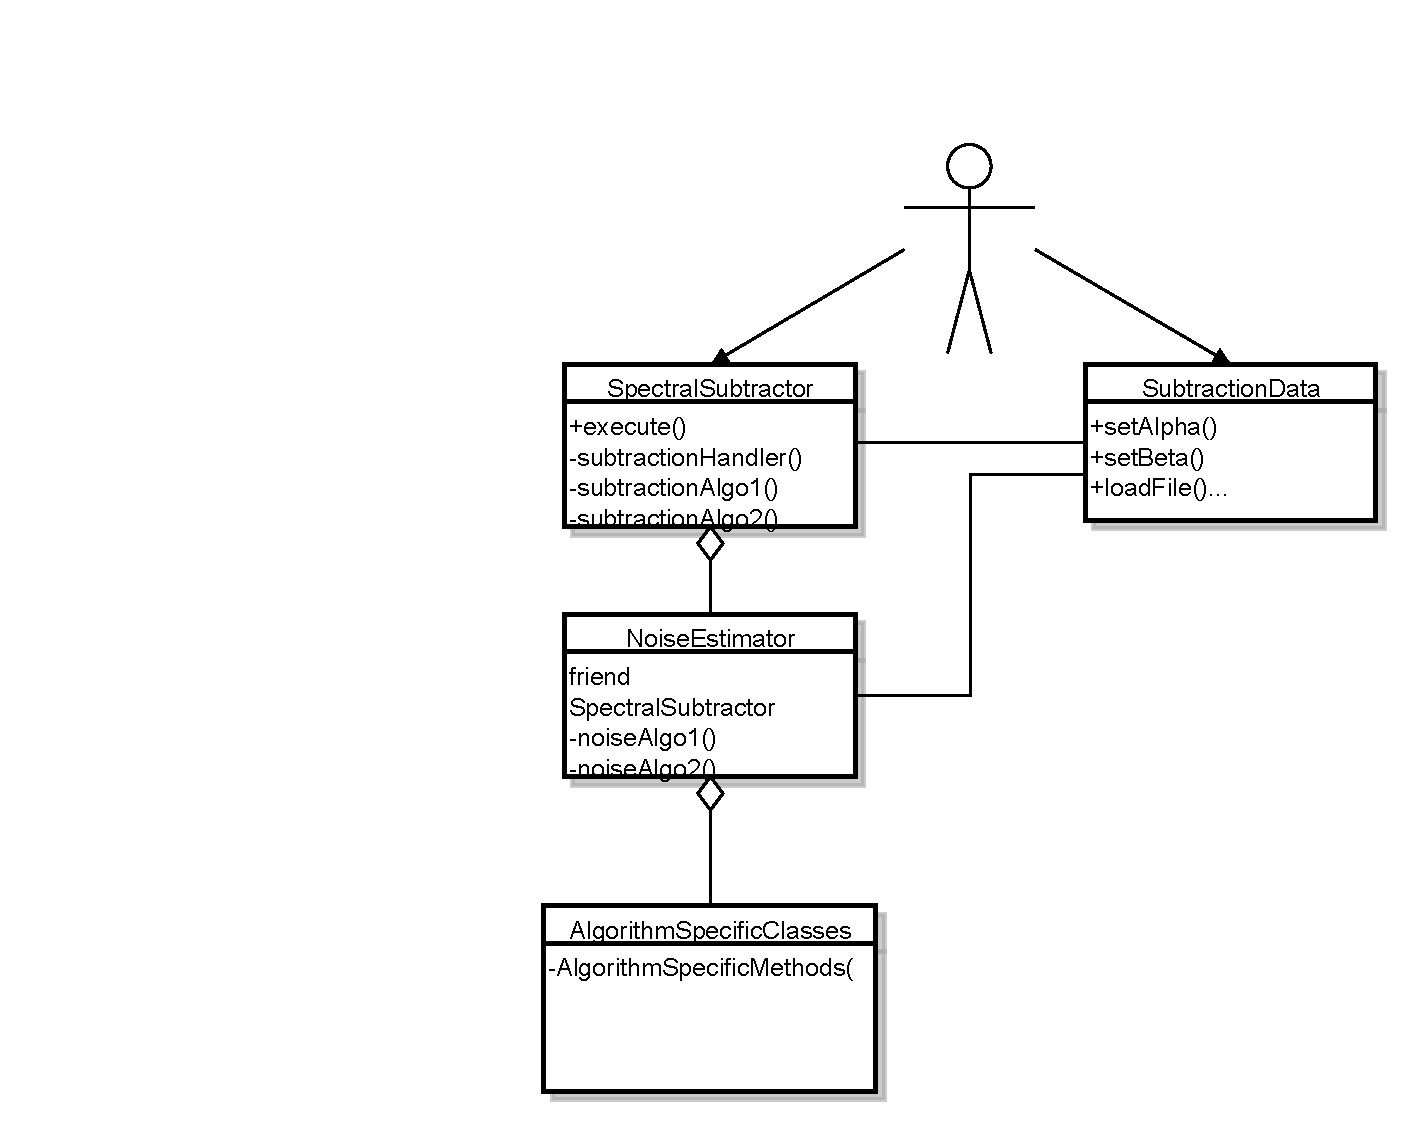
\includegraphics[scale=0.5]{old.pdf}
\caption{First organization of the library}
\label{diag_api_chords}
\end{center}
\end{figure}
The problem is that the data and the algorithms were intertwined. This could have caused problems when trying to thread. Also, the \texttt{SpectralSubtractor} and \texttt{NoiseEstimator} had to be friend with \texttt{SubtractionData}, which held many of the parameters required to perform the algorithms, like the number of iterations, etc.
Finally, the user had to manipulate two different objects, which causes unneeded clutter in the code.
\paragraph{Mid-internship reorganisation}
I then decided to refactor my code, by taking a modular approach, that would be more logical.
The user mostly interacts with the \texttt{SubtractionManager} object. This object holds : 
\begin{itemize}
\item The audio data.
\item Methods for loading an audio buffer, or a raw audio file.
\item A method to read parameters from a configuration file.
\item Methods to manage the Fourier transform.
\item Handlers to call if there is a change of data, or FFT size.
\item Methods to set general parameters, like the number of iterations, or the usage of the overlap-add method.
\item Two very important objects, of base class \texttt{Estimation} and \texttt{Subtraction}, and the associated getters and setters.
\end{itemize}
The \texttt{Estimation} and \texttt{Subtraction} objects hold the algorithm implementation. This reduces memory consumption, because only the wanted algorithm and needed implementation details are loaded, versus the previous approach where every algorithm had to be initialized. To permit a good memory management, I used a \brand{C++11} smart pointer \texttt{std::shared\_ptr} to keep them.

An example of initialization would be : 
\begin{lstlisting}
SubtractionManager s_mgr(fft_size, sampling_rate);
SimpleSpectralSubtraction* sub_algo = new SimpleSpectralSubtraction(s_mgr);
// Here we set algorithm-specific parameters.
// For instance they are not present in GeometricSpectralSubtraction class
sub_algo->setAlpha(data->alphaBsc); 
sub_algo->setBeta(data->betaBsc);
s_mgr.setSubtractionImplementation(std::shared_ptr<Subtraction>(sub_algo));
\end{lstlisting}

The \texttt{Estimation} and \texttt{Subtraction} objects are functors.

\begin{figure}[h]
\begin{center}
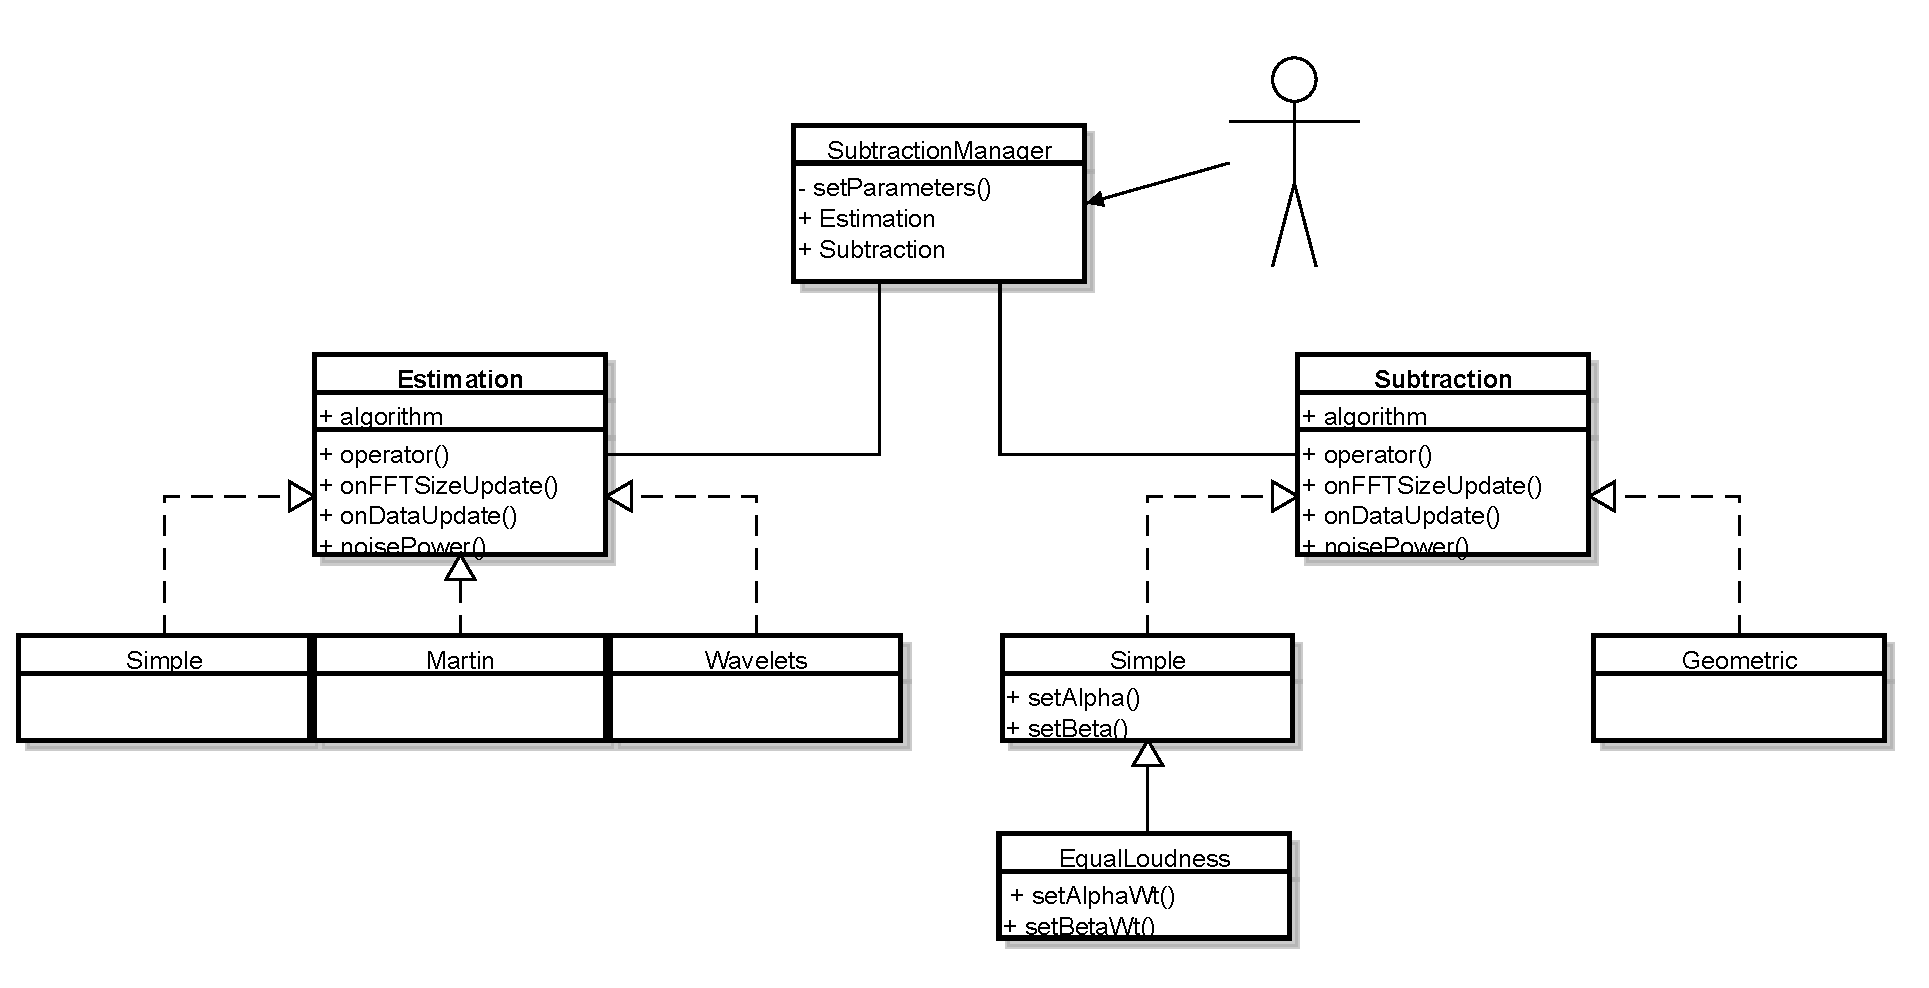
\includegraphics[scale=0.5]{base.pdf}
\caption{Current organization of the library}
\label{diag_api_chords}
\end{center}
\end{figure}

Finally, a very important algorithm is \texttt{SubtractionManager::execute()} because it is the one that gets called when the data and parameters are ready.

The code is very short : 
\begin{lstlisting}
for (auto iter = 0U; iter < iterations(); ++iter)
{
	for (auto sample_n = 0U; sample_n < getLength(); sample_n += getFrameIncrement())
	{
		copyInput(sample_n);
		forwardFFT();

		if(dataSource() == DataSource::File && sample_n == 0)
			onDataUpdate();

		// Noise estimation
		(*getEstimationImplementation())(spectrum());

		// Spectral subtraction
		(*getSubtractionImplementation())(spectrum(), 
			getEstimationImplementation()->noisePower());

		backwardFFT();
		copyOutput(sample_n);
	}
}
\end{lstlisting}
\subsubsection{Easy way to compare algorithms}
stuff
\paragraph{Technologies used}
stuff
\subsubsection{Implementation of an English acoustic and language model}
\paragraph{Technologies used}
stuff
\subsubsection{Evaluation}
\paragraph{Signal-level evaluation}
stuff
\paragraph{Word-level evaluation}
stuff
\subsubsection{Making the processed signal listenable}
\subsection{Research work}
\subsubsection{First idea to improve spectral subtraction}
\paragraph{Kansai joint conference}
stuff
\paragraph{Evaluation}
stuff
\subsubsection{Second idea to improve spectral subtraction}
\paragraph{Evaluation}